
%%%%%%
%
% $Autor: Wings $
% $Datum: 2020-01-18 11:15:45Z $
% $Pfad: githubtemplate/Template/report/rename.tex $
% $Version: 4620 $
%
%
% !TeX encoding = utf8
% !TeX root = Rename
% !TeX TXS-program:bibliography = txs:///bibtex
%
%%%%%%


\chapter{Portenta Cat. M1/NB IoT GNSS Shield)}


Arduino is a prestigious open-source electronics platform that seamlessly integrates user-friendly hardware and software, making it highly appealing to inventors, hobbyists, engineers, students, and professionals alike. At the heart of this platform is a versatile microcontroller, a mini-computer, that can be programmed and manipulated to interact with external signals from a wide variety of modules, including sensors and actuators, resulting in a wide array of control systems and interactive setups. \cite{Arduino2024Guide} 
\newline
Part of the appeal of Arduino is its commitment to making technology accessible to beginners. This is exemplified in the Arduino integrated development environment (IDE), which provides a streamlined, beginner-friendly programming environment. The IDE assists users in developing and uploading code to the Arduino microcontroller.
In summary, Arduino stands as a beacon for the open-source movement in electronics and has played a pivotal role tech-educational contexts, providing an easy-to-understand yet powerful platform for exploring the world of electronics and computer programming. \cite{Arduino2024Guide}

\section{Introduction}
The Portenta Cat. M1/NB IoT GNSS-Shield allows you to improve the connectivity capabilities of your Portenta H7 applications. The Shield uses a Thales Cinterion TX62 wireless module designed for high-efficiency, low-power IoT applications to ensure optimized bandwidth and performance. 
\\The Portenta Cat. M1/NB IoT GNSS-Shield combines with the strong edge computing performance of the Portenta H7 and enables the development of asset tracking and remote monitoring applications in industrial settings as well as in agriculture, public facilities and smart cities. The Shield offers a cellular connection for both Cat. M1 and NB-IoT networks with the option to use eSIM technology. Easily track your valuable assets across the city worldwide with your choice of GPS, GLONASS, Galileo or BeiDou.
\newline
The following below figures shows a Portenta Cat. M1/NB IoT GNSS Shield \cite{ArduinoPortentaStore:2024}

\begin{figure}
	\begin{center}
		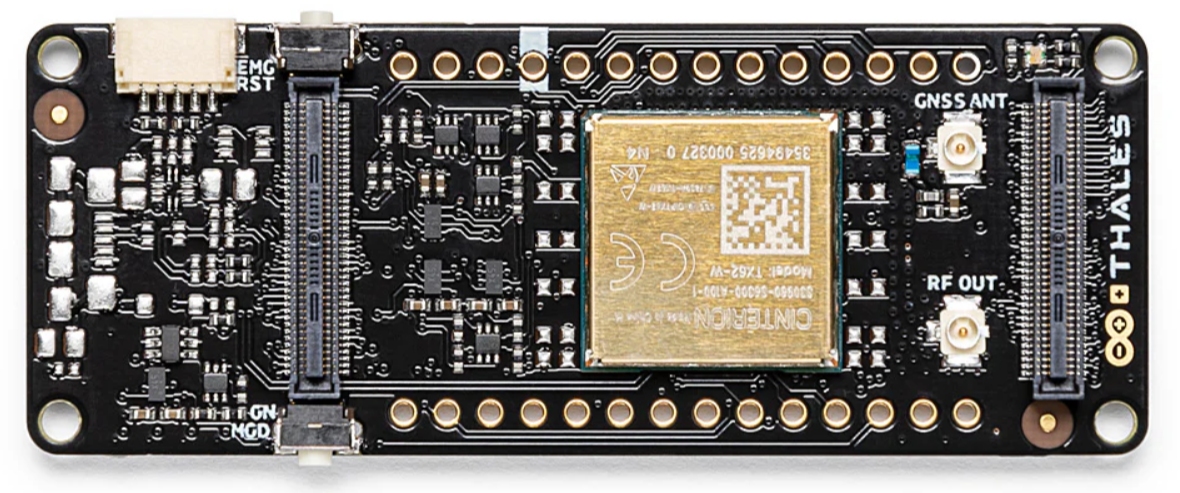
\includegraphics[width=0.7\linewidth]{Images/PotentaIoTGNSSShield/BoardFront.png}
		\label{BoardFront}
	\end{center}
\end{figure}

\begin{figure}
	\begin{center}
		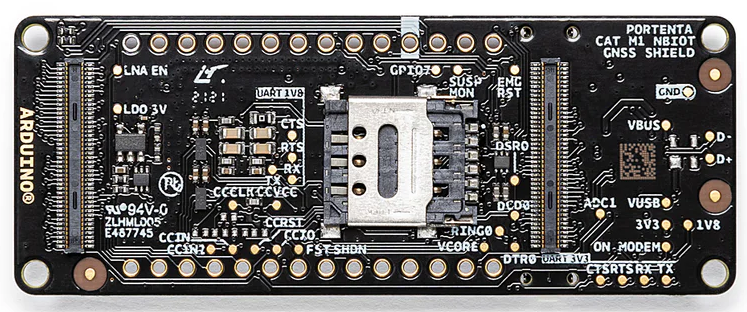
\includegraphics[width=0.7\linewidth]{Images/PotentaIoTGNSSShield/BoardBack.png}
		\caption{Portenta Cat. M1/NB IoT GNSS-Shield}
		\label{BoardBack}
		\cite{ArduinoPortentaStore:2024}
	\end{center}
\end{figure}

\section{Portenta Cat. M1/NB IoT GNSS Shield}

The Arduino Portenta Cat. M1/NB IoT GNSS Shield is designed to enhance the connectivity and localization capabilities of your Portenta or MKR boards. Portenta Cat. M1/NB IoT GNSS Shield is very small 66mm × 25.4mm in size and 9g in weight. It is a low power consumption board and operate normally on 3.3 V. Arduino Portenta Cat. M1/NB IoT GNSS Shield can still utilize UART, I2C, SPI communication protocols by connecting external devices to the appropriate pins on the Portenta board communication It is designed to provide reliable connectivity to the Portenta family of boards. It incorporates Cinterion TX62 wireless module for Cellular connectivity and provides connectivity to both Cat.M1 and NB-IoT networks. Also it supports GNSS capabilities for real-time positioning. The table below ~\ref{tab:TechSpec} shows the technical specifications of Portenta Cat. M1/NB IoT GNSS Shield. \cite{ArduinoPortenta:2024}

\begin{table}[ht]
	\centering
	\begin{tabular}{|>{\raggedright\arraybackslash}m{4cm}|>{\raggedright\arraybackslash}m{10cm}|}
		\hline
		\textbf{Connectivity} & Cinterion TX62 wireless module; NB-IoT - LTE CAT.M1; 3GPP Rel.14 Compliant Protocol LTE Cat. M1/NB1/NB2; UMTS BANDS: 1 / 2 / 3 / 4 / 5 / 8 / 12(17) / 13 / 18 / 19 / 20 / 25 / 26 / 27 / 28 / 66 / 71 / 85; LTE Cat.M1 DL: max. 300 kbps, UL: max. 1.1 Mbps; LTE Cat.NB1 DL: max. 27 kbps, UL: max. 63 kbps; LTE Cat.NB2 DL: max. 124 kbps, UL: max. 158 kbps \\
		\hline
		\textbf{Short Messaging Service (SMS)} & Point-to-point mobile terminated (MT) and mobile originated (MO) Text Mode; Protocol Data Unit (PDU) Mode \\
		\hline
		\textbf{Localization Support} & GNSS capability (GPS/BeiDou/Galileo/GLONASS) \\
		\hline
		\textbf{Dimensions} & 66 mm x 25.4 mm \\
		\hline
		\textbf{Other} & Embedded IPv4 and IPv6 TCP/IP stack access; Internet Services: TCP server/client, UDP client, DNS, Ping, HTTP client, FTP client, MQTT client Secure Connection with TLS/DTLS Secure boot \\
		\hline
		\textbf{Operating Temperatures} & -40° C to +85° C (-104° F to 185°F) \\
		\hline
	\end{tabular}
	\caption{Technical Specifications of Portenta Cat. M1/NB IoT GNSS-Shield}
	\label{tab:TechSpec}
	\cite{ArduinoPortenta:2024}
\end{table}

\subsection{Board Topology}

The figure ~\ref{BoardPinout} represents the Pinout details of Portenta Cat. M1/NB IoT GNSS Shield Board. The Arduino Portenta Cat. M1/NB IoT GNSS Shield requires a Portenta/MKR host board to operate. Power to the Arduino Portenta Cat. M1/NB IoT GNSS Shield is provided by the host Portenta board via the highdensity connector.
As can be seen from the figure, the pins A0 to A6 represents analog pins and D0 to D14 represents the digital pins. The ground pins (GND) are denoted in black color and power pins in red color. Also there is a RESET pin in the board. We can trigger the reset in the board by using Push-button switch either manually else programmable reset. VIN is the input voltage pin. This pin is used to power the Portenta Cat. M1/NB IoT GNSS Shield along with Portenta H7 board when no power source in portenta boards. The 3v3 represents 3.3 volts output voltage pin and +5V pin is also a output voltage pin which outputs 5V from the board when powered using portenta host board or using the VIN pin. \cite{ArduinoPortenta:2024}
\\The figure ~\ref{TopView} shows the Top View of Portenta Cat. M1/NB IoT GNSS Shield Board with the components listed in the table ~\ref{tab:TableTopView} 
The figure ~\ref{BottomView} shows the Top View of Portenta Cat. M1/NB IoT GNSS Shield Board with the components listed in the table ~\ref{tab:TableBottomView} \cite{ArduinoPortenta:2024}


\begin{figure}[H]
	\begin{center}
		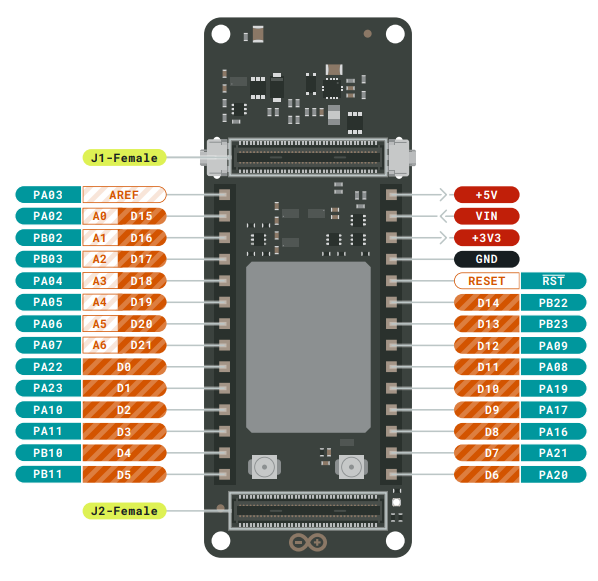
\includegraphics[width=0.7\linewidth]{Images/PotentaIoTGNSSShield/PortentaIoTGNSSShieldpinouts.png}
		\caption{Portenta Cat. M1/NB IoT GNSS Shield Pinout}
		\label{BoardPinout}
		\cite{ArduinoPortenta:2024}
	\end{center}
\end{figure}

\begin{figure}[H]
	\begin{center}
		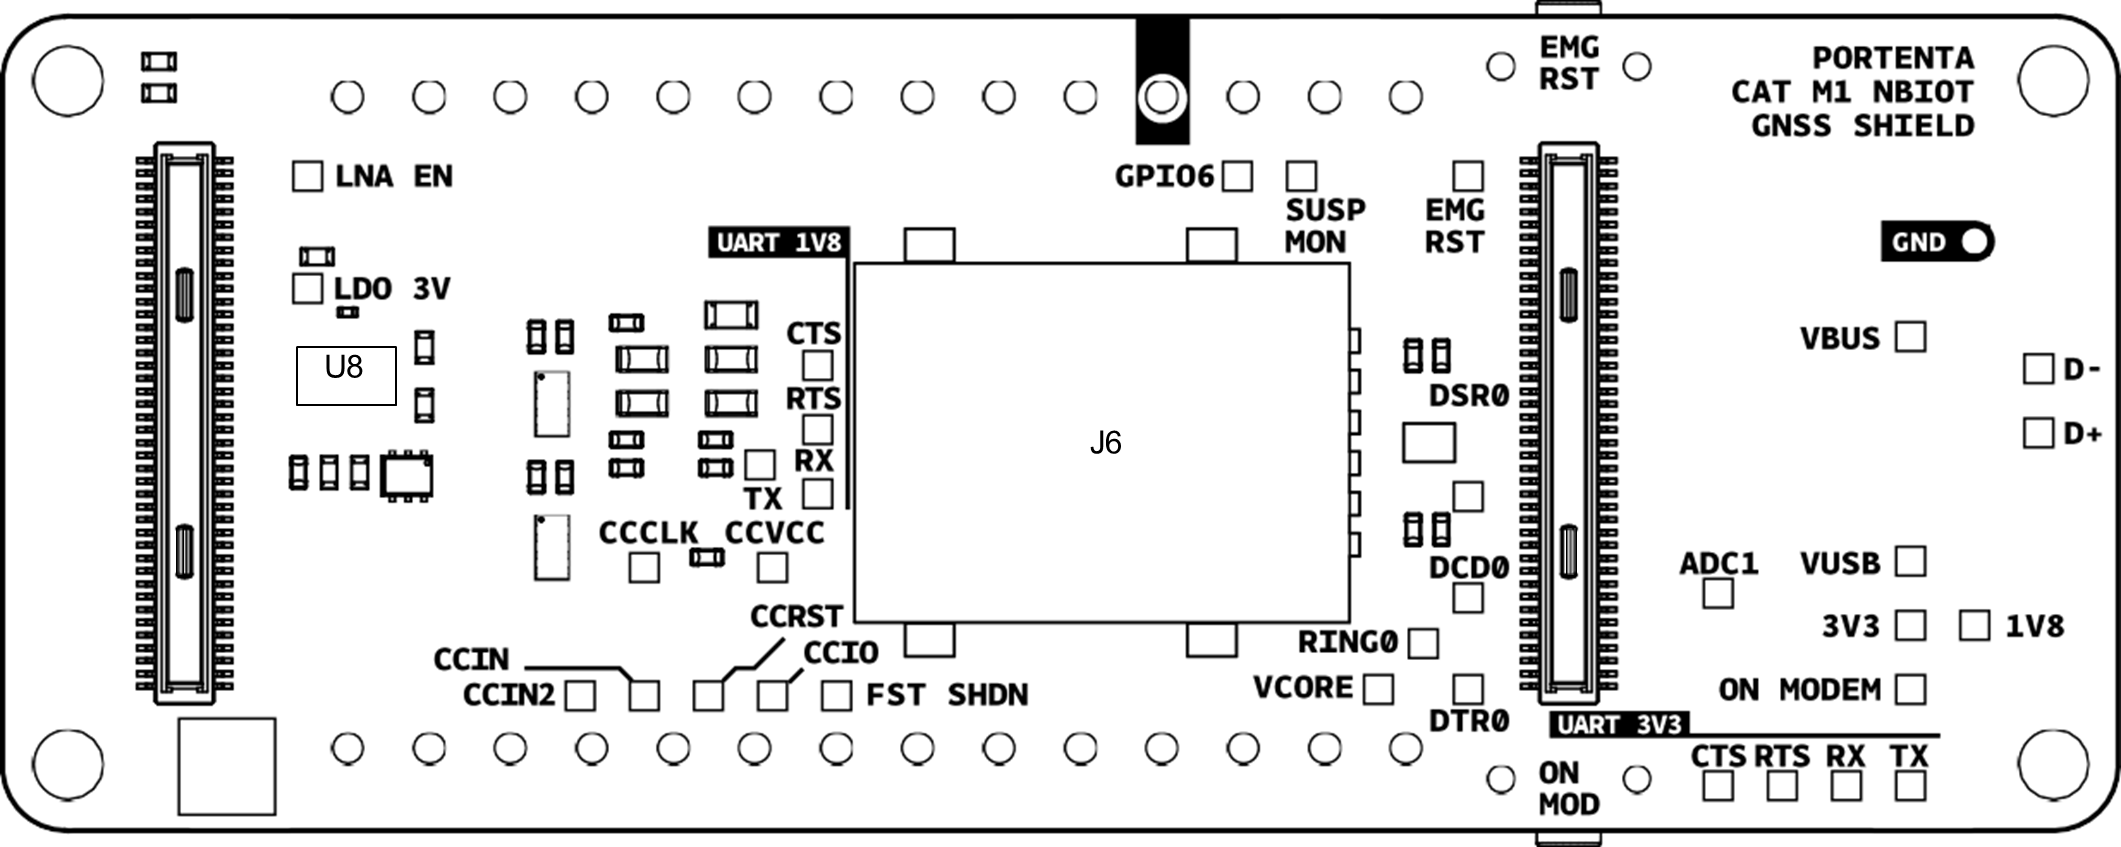
\includegraphics[width=0.7\linewidth]{Images/PotentaIoTGNSSShield/TopView.png}
		\caption{Portenta Cat. M1/NB IoT GNSS Shield Top View}
		\label{TopView}
	\end{center}
\end{figure}

\begin{table}[ht]
	\centering
	\begin{tabular}{|c|l|}
		\hline
		\textbf{Ref} & \textbf{Description}\\
		\hline
		DL1 & SMLP34RGB2W3 RGB LED \\
		\hline
		PB1 & TL3340AF160QG Mode Select button \\
		\hline
		U1  & TX62-W Cellular-GNSS Module \\
		\hline
		J1,12 & Female High Density Connector \\
		\hline
		PB2 & TL3340AF160QG Reset button \\
		\hline
		U2,U5,U7  & 74LVCH2T45GT Level Translator \\		
		\hline
	\end{tabular}
	\caption{Portenta Cat. M1/NB IoT GNSS Shield Top View Component Desription}
	\label{tab:TableTopView}
\end{table}

\begin{figure}[H]
	\begin{center}
		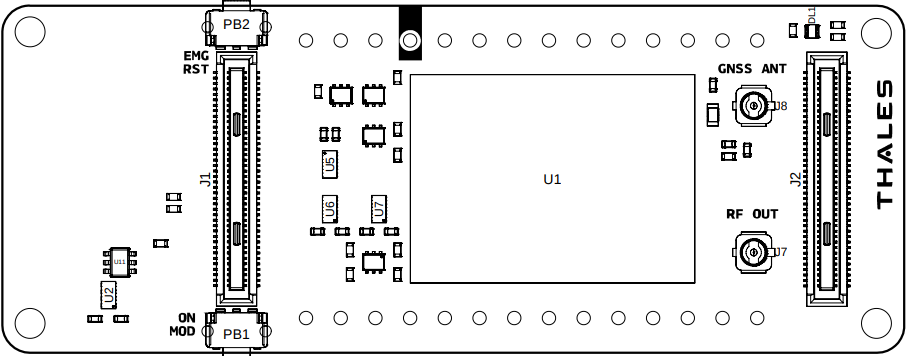
\includegraphics[width=0.7\linewidth]{Images/PotentaIoTGNSSShield/BottomView.png}
		\caption{Portenta Cat. M1/NB IoT GNSS Shield Bottom View}
		\label{BottomView}
	\end{center}
\end{figure}

\begin{table}[ht]
	\centering
	\begin{tabular}{|c|l|}
		\hline
		\textbf{Ref.} & \textbf{Description} \\
		\hline
		J3, J4 & Male High Density Connectors \\
		\hline
		J6 & SIM8060-6-0-14-00-A Hinged Nano SIM card module \\
		\hline
		J7 & U.FL-R-SMT-1(60) micro UFL Cellular Antenna Connector \\
		\hline
		J8 & U.FL-R-SMT-1(60) micro UFL GNSS Antenna Connector \\
		\hline
		U3,U4,U6 & 74LVCH2T45GT Level Translator \\
		\hline
		U8 & TC1185-3.0VCT713 3V 150mA LDO IC \\
		\hline
	\end{tabular}
	\caption{Portenta Cat. M1/NB IoT GNSS Shield Bottom View Component Description}
	\label{tab:TableBottomView}
\end{table}


	\subsection{Features} \cite{ArduinoPortenta:2024}
	\begin{itemize}[leftmargin=*]
		\item \textbf{Cinterion TX62 wireless module}
		\begin{itemize}[leftmargin=*]
			\item Cellular connectivity and positioning support
			\item Embedded IPv4 and IPv6 TCP/IP stack access
			\item Internet Services
			\begin{itemize}[label=--]
				\item TCP server/client
				\item UDP client
				\item DNS
				\item Ping
				\item HTTP client
				\item FTP client
				\item MQTT client Secure Connection with TLS/DTLS Secure boot
			\end{itemize}
		\end{itemize}
		
		\item \textbf{Cellular Connectivity}
		\begin{itemize}[leftmargin=*]
			\item LTE Cat. M1/NB1/NB2
			\item 3GPP Rel.14 Compliant Protocol LTE Cat. M1/NB1/NB2 
			\begin{itemize}[label=--]
				\item UMTS BANDS: 1 / 2 / 3 / 4 / 5 / 8 / 12 / 13 / 18 / 19 / 20 / 25 / 26 / 27 / 28 / 66 / 71 / 85
			\end{itemize}
			\item {LTE Bands}
			\begin{itemize}[label=--]
				\item LTE Cat.M1 DL: max. 300 kbps, UL: max. 1.1 Mbps
				\item LTE Cat.NB1 DL: max. 27 kbps, UL: max. 63 kbps
				\item LTE Cat.NB2 DL: max. 124 kbps, UL: max. 158 kbps
			\end{itemize}
			
			\item {Short Messaging Service (SMS)}
			\begin{itemize}[label=--]
				\item Point-to-point mobile terminated (MT) and mobile originated (MO)
				\item Text Mode
				\item Protocol Data Unit (PDU) Mode
			\end{itemize}

		\end{itemize}
				
		\item \textbf{Positioning Support}
		\begin{itemize}[leftmargin=*]
			\item Multiple GNSS Support
			\begin{itemize}[label=--]
				\item GPS
				\item GLONASS
				\item Galileo
				\item BeiDou
			\end{itemize}
			\item MKR and Portenta Compatible
			\begin{itemize}[label=--]
				\item MKR requires headers
			\end{itemize}
		\end{itemize}
	\end{itemize}


\subsection{Compabilities} \cite{ArduinoPortenta:2024}
The following \textbf{software tools} allow you to program your board both online and offline.
\begin{itemize}
	\item Arduino IDE
	\item Arduino CLI
	\item Web Editor
\end{itemize}
The \textbf{hardware} listed below is compatible with this product
\begin{itemize}
	\item Portenta Breakout
	\item Portenta H7
	\item Portenta H7 Lite
	\item Portenta H7 Lite Connected
\end{itemize}

\subsection{GNSS Capabilities}

The Arduino Portenta Cat M1/NB IoT GNSS Shield supports precise location tracking and navigation through multiple GNSS systems. \cite{ArduinoPortenta:2024}

\begin{itemize}
	\item \textbf{Supported GNSS Systems}: The shield supports four major GNSS constellations: GPS (Global Positioning System), GLONASS (Global Navigation Satellite System), Galileo, and BeiDou.
	\item \textbf{NMEA Protocol}: GNSS information is transmitted using the NMEA (National Marine Electronics Association) protocol, a standard for interfacing marine electronics.
	\item \textbf{Antenna Requirements}: An active GNSS antenna can be connected via the micro UFL connector (J8). The antenna should have a bias voltage of 3.0V and an input impedance of 50$\Omega$. To ensure compatibility with all GNSS systems, the antenna should support frequency bands over the 1559 - 1606 MHz range.
\end{itemize}
GNSS and cellular services cannot be used simultaneously. \cite{ArduinoPortenta:2024}

\subsection{GSM Capabilities}

The Arduino Portenta Cat M1/NB IoT GNSS Shield provides robust cellular connectivity through its GSM features, making it suitable for a wide range of IoT applications. \cite{ArduinoPortenta:2024}

\begin{itemize}
	\item \textbf{TX62-W Module}: The shield uses the TX62-W Module (U1) to access various cellular networks, supporting LTE Cat M1 and NB-IoT technologies.
	\item \textbf{External Antenna}: It is possible to connect an external cellular antenna via the micro UFL connector (J7). The input impedance for the cellular antenna is 50$\Omega$.
	\item \textbf{Data Transmission}: Supports both SMS and data transfer functionalities. SMS messages can be stored in the SIM card module.
	\item \textbf{AT Commands}: The modem can be controlled and configured using AT commands, allowing for precise management of the module’s functions.
	\item \textbf{Status Indicator}: Modem status is indicated by the RGB LED (DL1), providing visual feedback on the module’s operation.
	\item \textbf{SIM Card Integration}: A standard SIM card slot allows for easy integration with mobile network services. Users need to configure the APN and PIN settings in their code.
	\item \textbf{IPv4 and IPv6 Support}: Supports both IPv4 and IPv6, ensuring future-proof connectivity.
\end{itemize}
The Portenta Cat. M1/NB IoT GNSS Shield requires a physical nano-SIM for cellular connectivity. \cite{ArduinoPortenta:2024}

\section{Portenta Cat. M1/NB IoT GNSS Shield Application Examples}


\textbf{Arduino Portenta Cat. M1/NB IoT GNSS Shield} shield can connect to your Portenta/MKR board enabling a wide range of applications. \cite{ArduinoPortenta:2024}
\begin{itemize}
	\item \textbf{Global Asset Tracking:} The Arduino Portenta Cat. M1/NB IoT GNSS Shield provides connectivity to four major satellite positioning networks, allowing you to track your inventory reliably. The multi-band cellular connectivity ensures you get live updates on your inventory nearly anywhere in the world.
	\item \textbf{Remote Node Monitoring:} The Arduino Portenta Cat. M1/NB IoT GNSS Shield can relay geo-tagged data from local sensors located worldwide to provide real-time insight for increasing your business revenues.
	\item \textbf{Fleet Management:} Manage your Mobility as a Service (MaaS) solution across the city or between borders. Track, analyze, and dynamically manage your fleet to optimize fuel usage, increase customer satisfaction, and reduce transport times. Enable predictive maintenance and remote diagnostics to ensure your business runs smoothly with minimal downtime.
\end{itemize}

\chapter{First Step with Portenta Cat. M1/NB IoT GNSS Shield}

\section{Introduction}
In this chapter, we will be looking how to use GSM networks to connect to a server and display it's content in the serial monitor. \cite{ArduinoPortentaSketch:2024}

\subsection{Configuration}
First, we need to install Arduino Mbed OS Portenta core in the IDE platform and connect the Arduino Portenta Cat. M1/NB IoT GNSS shield to the Arduino Portenta H7 using HD connectors. Then we need to connect with the GSM network using NB IoT or Cat. M1 technology and print the website's HTML content in the Serial Monitor.  	

\subsection{Requirements}
\begin{itemize}
	\item Arduino IDE (online or offline)
	\item Portenta H7
	\item Portenta Cat. M1/NB IoT GNSS Shield
	\item Dipole Antenna (connected to the RF OUT antenna connector on the top side of the shield)
	\item SIM card (standard pre-paid or post-paid SIM card that supports Cat M1 or NB-IoT connectivity, along with details of APN settings and PIN code usually 0000 or 1234. These are usually provided by your SIM card provider)
\end{itemize}

\subsection{Procedures}

First insert the SIM card into the SIM card slot at the bottom of the Portenta Cat. M1/NB IoT GNSS Shield \cite{ArduinoPortentaSketch:2024}. The figure ~\ref{DipoleAntenna} shows where to connect the dipole antenna to the shield. It should connect to the antenna connector marked RF OUT.
\begin{figure}
	\begin{center}
		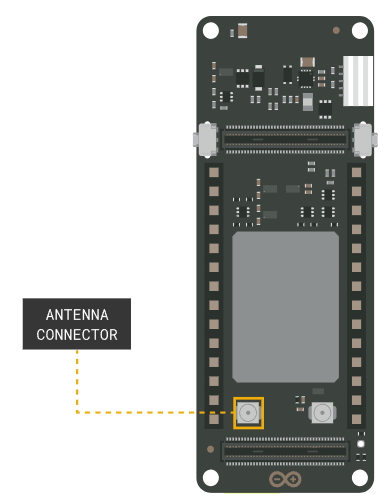
\includegraphics[width=0.7\linewidth]{Images/PotentaIoTGNSSShield/AntennaConnector.png}
		\caption{Arduino Mbed OS Portenta core installation in Arduino IDE}
		\label{DipoleAntenna}
	\end{center}
\end{figure}
\\
Now connect the shield to the Portenta H7. Do this by attaching it to the HD connectors at the bottom of the Portenta H7 board. The figure ~\ref{BoardShieldConnection} shows the top and bottom high density connectors on the shield are connected to the corresponding ones on the lower side of the H7 board. Press firmly to let it snap in. Once attached, plug the Portenta H7 into your computer using a USB-C cable.
\begin{figure}
	\begin{center}
		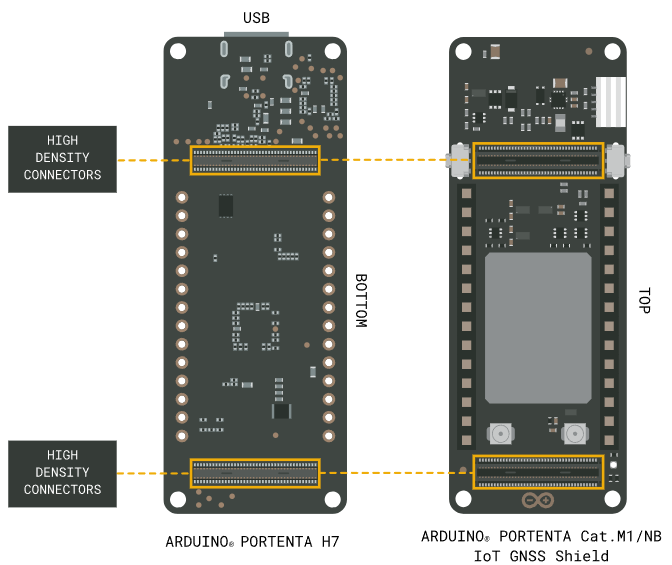
\includegraphics[width=0.7\linewidth]{Images/PotentaIoTGNSSShield/BoardShieldHDConnectors.png}
		\caption{Arduino Mbed OS Portenta core installation in Arduino IDE}
		\label{BoardShieldConnection}
	\end{center}
\end{figure}

\subsubsection{Arduino IDE}
Make sure that the latest Arduino Mbed OS Portenta core installed. We can install it with the board manager under \SHELL{Tools > Board > Board Manager} as shown in figure ~\ref{CoreInstallation} With the core installed and the board selected, navigate to \SHELL{File > Examples > GSM > GSMClient}. The listing reference ~\ref{lst:GSMclientCode} shows the example sketch we will use to test out the Cat. M1 or NB IoT connection. \cite{ArduinoPortentaSketch:2024}

\begin{comment}
\begin{code}
	% Include a specific range of lines from the C++ file
	\lstinputlisting[language=C++, firstline=1, lastline=47, label={lst:GSMclientCode}]{../Code/PortentaIOTGNSSShield/GSMClientCode.cpp}	
\end{code}

\end{comment}

\begin{figure}[h]
	\centering
	\lstinputlisting[language=C++, firstline=1, lastline=47]{../Code/PortentaIOTGNSSShield/GSMClientCode.cpp}
	\caption{GSM Client Code for Portenta IoT GNSS Shield}
	\label{lst:GSMclientCode}
\end{figure}


\begin{figure}
	\begin{center}
		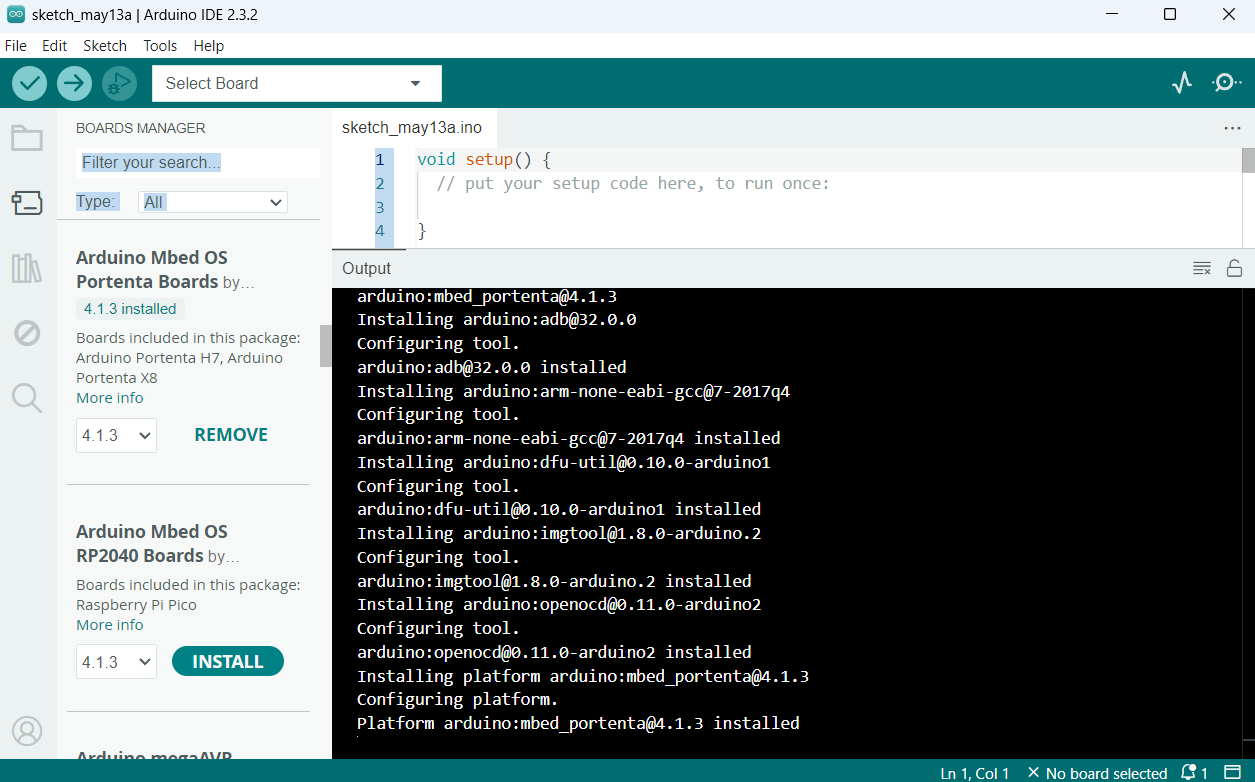
\includegraphics[width=0.7\linewidth]{Images/PotentaIoTGNSSShield/CoreInstallation.png}
		\caption{Arduino Mbed OS Portenta core installation in Arduino IDE}
		\label{CoreInstallation}
	\end{center}
\end{figure}

\subsubsection{Programming the Board}
Go to the \PYTHON{arduino\_secrets.h} tab that opens with the example and enter the PIN of the SIM card you are using into the \SHELL{SECRET\_PIN} variable. Check your SIM card provider's mobile APN (e.g., "online.provider.com") and save it inside \SHELL{SECRET\_APN}.
\\
\textbf{NOTE}:
An Access Point Name (APN) is a gateway between a GSM, GPRS, 3G or 4G mobile network and another computer network, frequently the public Internet
The username and password depend on your provider; these are required to authenticate with the APN gateway. These values can usually be found by searching online for APN credentials and provider names. Sometimes they can be left blank.
\\
Using \PYTHON{GSM.begin()} will make the GSM module start with the PIN and APN entered in \verb|arduino_secrets.h|. To decide whether to use NB IoT or Cat. M1 technology, you need to change the last argument. Use either \verb|CATNB| for NB IoT or \verb|CATM1| for Cat. M1. If you are unsure what technology to use, check with your SIM card provider.
Using \PYTHON{GSM.begin()} will make the GSM module start with the PIN and APN entered in \PYTHON{arduino\_secrets.h}. To decide whether to use NB IoT or Cat. M1 technology, you need to change the last argument. Use either \verb|CATNB| for NB IoT or \verb|CATM1| for Cat. M1. If you are unsure what technology to use, check with your SIM card provider.


	\SHELL{GSM.begin(pin, apn, username, pass, CATNB);}


When the GSM module starts, you can connect to a remote server using the server URL. The port to connect to is also defined; it is set to \texttt{80} by default.

	\SHELL{client.connect(server, port);}


\subsection{Result of Sketch}
After finishing this setup, compile and upload the program. You should see the HTML content of the server printed in the Serial Monitor. The server is set as doc.arduino.cc as default. \cite{ArduinoPortentaSketch:2024}


	

